\begin{savequote}[75mm]
It might be urged that when playing the ``imitation game'' the best strategy for the machine may possibly be something other than imitation of the behaviour of a man. This may be, but I think it is unlikely that there is any great effect of this kind.
\qauthor{Alan Turing}
\end{savequote}

\chapter{Robustness of the Luna Rating System}

\section{The Smarts Rating as a Proxy for Intelligence}

The Luna Rating System is only effective as a test if Smarts Ratings genuinely reflect intelligence. Without appropriate safeguards, Smarts Ratings can quickly lose their integrity. To illustrate this potential danger, consider a version of LRS that initializes all new players with a Smarts Rating of $50$. In the early days of LRS, if this initialization is known to all players, the strategy of always guessing $50$ will do quite well. In fact, if all players guess rationally, no rating will ever deviate from $50$, and every Luna Game will end in a tie. As more players join the system, if the equilibrium has already been fixed at this constant, no rational force will make it budge. This outcome would render the version of LRS unusable for testing intelligence and uninteresting for players. Clearly LRS must be implemented with care.

This chapter studies the extent to which a player's Smarts Rating may be different from the player's intelligence. I formalize intelligence to be the expected ``Actual Guess'' made by an opponent of the player's Smarts Rating. Trouble arrives when players choose to give a ``Reported Guess'' that is different from an Actual Guess. From this discrepancy emerges distance between the Smarts Rating and intelligence, i.e. error in Smarts Ratings. It is theoretically possible for Smarts Ratings to be arbitrarily far from intelligence; if all players report random or adversarial Guesses, Smarts Ratings will be meaningless. However, it is safe to assume that most players seek Luna Game wins, high Smarts Ratings, or both. With these motivations, there are several likely strategies that players may choose among. The robustness of LRS can be assessed through the analysis of these strategies and their cumulative effects on Smarts Ratings.

\subsection{Demonstrated Intelligence}

In considering the validity of Smarts Ratings, a natural question is whether the intelligence demonstrated by players during the Luna Game is indicative of ``actual'' intelligence. Assuming that players are capable of demonstrating intelligence through language in real life, it is clear that players may demonstrate intelligence during a Luna Game. But what if a player chooses not to demonstrate intelligence? What if a player is capable of answering with high intelligence, but decides to provide a subpar answer, perhaps out of laziness or misguided strategy? In this case, the Smarts Rating of the player may not reflect their capacity for intelligence. However, from the perspective of LRS as a test for intelligence, this possibility is not at all problematic. LRS is ultimately a test for \textit{demonstrated intelligence}. It evaluates the intelligence of responses, not the intelligence of respondents. Indeed, any test for intelligence is inherently an evaluation of demonstrated intelligence; it is impossible to assess anything else. 

\subsection{Reported and Actual Guesses}

If a player withholds a strong response in favor of a weak response, the withheld response is irrelevant for LRS. However, if a player withholds an honest guess of the opponent's Smarts Rating in favor of a dishonest one, this can have negative consequences for the validity of LRS. If a student fails an exam, that does not mean the exam has failed its purpose, but if an exam is graded incorrectly, its value is lost. Thus in studying the dynamics of Smarts Ratings, a distinction must be drawn between Reported Guesses and Actual Guesses. The system must be designed in such a way that Reported Guesses are equal to Actual Guesses as often as possible. I explore the consequences of misalignment below.


\subsection{Definitions and Notation}

Let $P$ be the set of all players in the LRS. Let $\mathcal{P}$ be a random variable that assumes values over $P$ with uniform probability. Let $SR \subseteq \mathbb{R}^+$ be the domain of Smarts Ratings. The definitions of Reported Guess and Smarts Rating are mutually dependent.

\theoremstyle{definition}
\begin{definition}{Reported Guess}\\
For players $p, p' \in P$, player $p$ has a \textit{Reported Guess} of the Smarts Rating of player $p'$, written as $G(p, p') \in SR$.
\end{definition}

\noindent The definition of Reported Guess assumes that players do not make decisions stochastically, nor based on their state. It is possible to weaken this assumption and arrive at similar conclusions.

\theoremstyle{definition}
\begin{definition}{Smarts Rating}\\
The \textit{Smarts Rating} of a player $p \in P$ is the expected Reported Guess of an opponent. This is written as $S(p) \triangleq E[G(\mathcal{P}, p)]$.
\end{definition}

\noindent The given definition of Smarts Ratings is an expectation rather than a quantity that depends on the number of Games played. This definition is expedient for theoretically evaluating the discrepancy between Smarts Ratings and intelligence. Later I provide simulations that probe the role of time in this discrepancy. Additionally, note that this definition does not preclude a player from playing herself, which is of course impossible in practice. Incorporating this observation into the definition would have no meaningful effect on results and would only muddle the analysis, hence the exclusion.

\theoremstyle{definition}
\begin{definition}{Actual Guess}\\
For players $p, p' \in P$, player $p$ has an \textit{Actual Guess} of the Smarts Rating of player $p'$, written as $G^*(p, p') \in SR$.
\end{definition}

\noindent The Actual Guess may or may not be different from the Reported Guess.

\theoremstyle{definition}
\begin{definition}{Intelligence}\\
The \textit{intelligence} of a player $p \in P$ is the expected Actual Guess of an opponent. This is written as $I(p) \triangleq E[G^*(\mathcal{P}, p)]$.
\end{definition}

\section{Theoretical Effects of Strategies on Smarts Rating Validity}

LRS presents two goals for players: to win Luna Games, and to achieve high Smarts Ratings. The spirit of the game encourages players to answer all questions as they would in a real world context, and to guess the Smarts Rating of an opponent in the same manner as they would evaluate the intelligence of a human. However, players may ignore the spirit of the game and adopt strategies that they think will maximize payoff in terms of both goals. They may also decide to focus on only one of the two goals, strategizing to maximize Luna Game wins at the expense of Smarts Ratings, or vice versa. If the Smarts Rating is to be used as a proxy for intelligence, the equivalence between the two must be robust to any likely player strategies.

\subsection{Honest Play}

If players always have Reported Guesses that are the same as their Actual Guesses, then Smarts Ratings will align with intelligences over time. This follows directly from the formalized definition of intelligence given above. Thus LRS designers should take every measure to encourage honest play.

\subsection{Single Priority Play}

One must always be prepared for players to ignore the spirit of the game and break any rules that aren't technically enforced. Honest play assumes that players give their best guess for any player's Smarts Rating. It also assumes that players present themselves as intelligently as possible with the aspiration of winning individual Luna Games. But what if a player cares only about Smarts Ratings and is indifferent towards the outcome of Luna Games? Or what if the opposite occurs, with a player ignoring Smarts Ratings and focusing only on winning Luna Games? In this section, I explore the system-level effects in both of these cases.

\subsubsection{Luna Game Win Maximization}

Suppose that a player is indifferent to her Smarts Rating and cares only to maximize her expected number of Luna Game wins. With the incentive of winning a game, it is clear that the player will provide a Reported Guess that is equal to her Actual Guess. The only aspect of the game that this player may manipulate is her responses. For example, if she currently has a very high Smarts Rating, she may provide responses that are indicative of a very low Smarts Rating, inducing a low guess from the opponent and increasing the probability of winning. The optimal strategy may be to oscillate between maximally intelligent responses and minimally intelligent ones, maintaining a Smarts Rating near the center of the range of possible ratings. 

In any case, strategizing by manipulating responses does not in any way jeopardize the validity of Smarts Ratings. As described above, LRS does not claim to be a test for capacity for intelligence; it can only be a test of demonstrated intelligence. If a human exhibits highly intelligent behavior one day and minimally intelligent behavior the next day, their overall intelligence is judged to be somewhere in between. As an average of play over time, the Smarts Rating captures this intuitive notion of intelligence better than any one-time evaluation could. Thus players may be able to ``game their opponents'' by oscillating the quality of their responses, but they will not be able to game the system.

\subsubsection{Smarts Rating Maximization}

Suppose that a player ignores Luna Game outcomes and strategizes to maximize her Smarts Rating at all costs. The best response strategy is clearly to respond as intelligently as possible at all times, which is in line with the spirit of LRS. However, if the player interprets Smarts Ratings as relative measures, the optimal guessing strategy is to give a Reported Guess of $0$ regardless of the opponent's play. This strategy is optimal because the player will perceive a slight benefit from a decrease in the opponent's rating. 

I assess the net impact of this Minimum Guessing strategy on LRS validity from two angles. First, to evaluate the likelihood that the strategy is adopted, I quantify the expected benefit of adopting this strategy for an individual player. I show that as a function of the number of players in the system, this benefit is so small that a player concerned only marginally with winning Luna Games will be better off playing honestly. Second, in the event that a player does adopt this strategy, I quantify the error that Minimum Guessing introduces to Smarts Ratings as a function of the number of players that adopt it.

Consider the Minimum Guessing strategy from the perspective of an individual player. If the player truly attaches zero value to a Luna Game win, then always guessing $0$ makes sense. But if the player cares even a marginal amount about wins, the personal benefit from guessing $0$ is unlikely to outweigh the cost. Let $p \in P$ be a player deciding between honesty and Minimum Guessing. Note that the Smarts Rating of $S(p)$ will be unchanged regardless, since $p$'s strategy choice will not affect the Guessing strategies of opponents. Let $s_1$ the mean Smarts Rating if $p$ Guesses honestly, where $N$ is the number of players in the system. We can express $s_1$ as
\begin{center}
\begin{math}
s_1 = \frac{1}{N}(\sum_{p' \in P}S(p')) = \frac{1}{N^2}(\sum_{p' \in P}(\sum_{p'' \in P}G(p'', p')))
\end{math}
\end{center}

\noindent Let $s_2$ be the mean Smarts Rating if $p$ instead uses the Minimum Guessing strategy. In this case, each Guess $G(p, p')$ in the expression of $s_1$ will change to $0$. Therefore the new mean Smarts Rating in this scenario will be 
\begin{center}
\begin{math}
s_2 = s_1 - \frac{1}{N^2}(\sum_{p' \in P} G(p, p'))
\end{math}
\end{center}
The relative benefit to the $p$ in choosing the Minimum Guessing strategy is thus \\
$\frac{1}{N^2}(\sum_{p' \in P} G(p, p'))$. For perspective, suppose that $p$ has Actual Guesses that are perfect, i.e. they match the Smarts Ratings of other players. Then the relative benefit is $\frac{1}{N}$ of the average Smarts Ratings of all players in the system.  As the number of players in the LRS increases, this change quickly becomes negligible. Thus any rational player with even the slightest desire to avoid losing every Luna Game will likely abstain from the Minimum Guessing strategy.

While the Minimum Guessing strategy is evidently subpar for players caring at all about winning, there may still be players who choose to adopt it. Suppose that there are $K$ such players, indexed $p_1, p_2, ..., p_K \in P$, with all other players adhering to Honest Guessing. I quantify the expected error introduced to the Smarts Rating of another player $p \in P$ as a result of these $K$ rogue players. Let $p \in P$. The most accurate Smarts Rating, i.e. the intelligence, is given by
\begin{center}
\begin{math}
I(p) = \frac{1}{N}(\sum_{p' \in P}(G^*(p', p)))
\end{math}
\end{center}
The Smarts Rating actually assigned to $p$ in this scenario is
\begin{center}
\begin{math}
S(p) = \frac{1}{N}(\sum_{p' \in P}(G(p', p))) = \frac{1}{N}((\sum_{p' \in P}(G^*(p', p)) - (\sum_{i=1}^K(G^*(p_i, p))))
\end{math}
\end{center}
Thus the total error introduced by these $K$ players is $\frac{1}{N}(\sum_{i=1}^K(G^*(p_i, p)))$. At a high level, this equation tells us that if half the players in the system use Minimum Guessing, then a player's Smarts Rating will be roughly half the player's intelligence. This impact suggests that LRS is tolerant to a small minority of Minimum Guessing players, but measures should be taken to discourage and prevent wide use of the strategy.

\subsection{Response Agnostic Play}

How should a first-time Luna Game player formulate her guess? There are several possible sources of information that she may utilize. She has her opponent's responses, and she may be able to estimate the intelligence of the opponent's responses based on experiences outside LRS. However, the responses and intelligence estimate alone are not enough to provide a guess; she also needs to understand the meaning and scale of a guess. Here LRS instructions may provide three sources of insight: the initialization value of Smarts Ratings, the domain of Smarts Ratings, and the distribution of Smarts Ratings for players currently in the system. In the extreme case, a player may ignore opponent responses completely and utilize only the statistics provided by LRS. How would such strategizing affect the validity of Smarts Ratings? This question is of import not only for first-time players, but also for experienced players who might incorporate these statistics into their overall strategies if they are available.

\subsubsection{Known Initialization}

As described in the introduction of this chapter, a known constant initialization value for Smarts Ratings could lead to an abrupt collapse in Smarts Ratings. Many early players would likely recognize that ($1$) new players have the same Smarts Rating and ($2$) most players are new, and therefore ($3$) the strategy of guessing the initialization value is highly effective. The result would be a quick collapse in Smarts Ratings to the initialization value, from which the system could not recover. 

There are three alternatives to initialization with a constant value. The first is initialization according to some predefined ``quiz''. This option is unattractive, not only because it primes players to think of intelligence in a particular way, but also because it induces players to ask similar questions to try to mimic the quiz. The second alternative is random initialization. While avoiding theoretical problems, this option has the practical downside of discouraging players who are randomly initialized low Smarts Ratings. It also makes the opponent's job of guessing first time players an arbitrary endeavor.

The third and preferable alternative to fixed initialization is to forgo initialization altogether. A player's Smarts Rating can be assigned \textit{after} her first Luna Game, and it will be equal to the guess of her opponent. With this configuration, there is no initialization that makes sense for players to guess as a default. The only downside of this approach is that the outcome of the first Luna Game loses meaning. To avoid discouraging experienced players, a Luna Game between a first time player and a non-first time player will result in a win for the latter, but will not be counted as a loss for the first time player. A Luna Game between two first time players will result in a tie. This third option is the one used in the implementation of LRS described in this thesis.

\subsubsection{Known Distribution}

A seemingly natural feature to include in an instantiation of LRS is the ability to see the distribution of all Smarts Ratings in the system. Revealing the distribution makes it possible for players to adopt guessing strategies that take advantage of this distribution. This is not inherently bad for LRS; for example, the strategy of randomly sampling from the distribution for guessing will preserve the distribution. However, other strategies involving the distribution can detrimentally affect the distribution. For example, suppose that a player's instinctive Actual Guess is the highest value presently in the distribution. The player may reason that the probability of her current opponent actually being the best player in the system is low, and therefore provide a guess that is lower than the maximum, even if the opponent actually is the best player. The net effect will be a collapsing towards the center of the distribution, as witnessed in the case of a fixed known initialization value.

The most extreme strategy that takes advantage of a known distribution is to always guess the mean Smarts Rating in the current distribution. It is clear that if all players adopted this strategy, all Smarts Ratings would converge to a constant. More realistic is the supposition that some players will judge opponents using percentiles, e.g. ``my opponent is smarter than $75$\% of other players'', and then map this judgment to the percentiles evident in the Smarts Ratings distribution, e.g. ``$75$\% of players have Smarts Ratings less than or equal to $55$, so my guess is $55$.'' This strategy uses the Quantile Function of the Smarts Rating distribution, and thus it is referred to as Quantile Guessing.

Let $Q : [0, 1] \to SR$ be the Quantile Function for the Smarts Rating distribution, and let $F_p : P \to [0, 1]$ be the ``player percentile function'' that $p$ uses to map other players to percentiles according. This function may be thought of as a cumulative distribution function over $\mathcal{G}_p = \{G(p, p') : p' \in P\}$, i.e. $F_p(p') = P[X \le G(p, p')]$ where $X \sim \mathcal{G}_p$. If player $p$ uses Quantile Guessing, her Reported Guess of player $p' \in P$ will be $G(p, p') = Q(F_p(p'))$. If Quantile Guessing is used by all players from the beginning of LRS, Smarts Ratings will again collapse to a constant. Early players will know that there are only a small number of possible values for Smarts Ratings and will guess by selecting one, which will quickly lead to the ratings converging to one value. It is less clear if Quantile Guessing is problematic once a wide distribution of Smarts Ratings has already been established by players of other strategies. For insight here, I turn to simulations.

\section{Simulations}

Thus far I have outlined the major Luna Game strategies and described their theoretical implications on the validity and volatility of Smarts Ratings. I next provide simulation results to further stress test LRS against various strategies. Simulations are necessary not only to corroborate the theory, but also to ask questions that cannot be cleanly answered otherwise. For example, whereas the strategies have only been discussed individually so far, simulations allow for a comprehensive study of combined strategies. The theoretical section also did not explore the amount of time required to reach each equilibrium; such questions are left to simulations. The resulting collection of theoretical and simulation insights lays a foundation for robust LRS design.

\subsection{Methods}

The recruitment of human players is pivotal to the success of LRS because it is not otherwise clear what form Actual Guess functions will take. For the purpose of simulations, I create $N$ simulated players and assign each a uniformly random value between $0$ and $100$. The Actual Guess function for a given player is created by adding random Gaussian noise $(\mu = 0, \sigma^2 = 5)$ to each of the initialized values. Thus a player's intelligence, defined as the expected Actual Guess, will be very close to the initialized random value for that player. The Reported Guess for each player varies according to the experiments, following one of the strategies described in ($2$). 

An experiment runs for $T$ time steps. At each time step, two players are randomly selected from the pool of all $N$ players. Each player reports her Reported Guess of the other's Smarts Rating, and each player's Smarts Rating is updated so that it is the mean of all previous Reported Guesses. After the $T$ time steps, the main dependent variable of interest is the $L_1$ error between players' Smarts Ratings and intelligences. I measure both the average error and the maximum error. For some strategies, the independent variable of interest is $N$, and for others it is $T$. If $N$ is kept constant, it is done so at $N=100$; if $T$ is kept constant, it is done so at $T = 1000$. All configurations are run $100$ times and averaged over the trials.

\subsection{Results}

\subsubsection{Baseline}

Since Smarts Ratings and intelligences are both on a scale from $0$ to $100$, one baseline for the $L_1$ distance between the two is achieved by assuming that all players give the same constant Reported Guess, such as $0$ (which would happen if all players use Minimum Guessing). Doing so would result in an expected error of $50$. Another baseline is given by the expected distance between two uniformly randomly selected points from the domain of Smarts Ratings. For two random variables $A_1$ and $A_2$ drawn independently from the uniform distribution over $[0, 100]$, let $B$ be a random variable given by $B = max(A_1, A_2)$, and let $C$ be a random variable given by $C = min(A_1, A_2)$. By symmetry, $E[100 - C] = E[B]$. Furthermore, the expected value of $B$ is half that of $C$ (this can be derived by conditioning on the values of $A_1$ and $A_2$), so $2E[B] = E[C] \implies E[C-B] = E[B]$. Now note that $B + (C-B) + (100-C) = 100$, so $3E[C-B] = 100 \implies E[C-B] = \frac{100}{3}$. Thus $33.33$ is one appropriate baseline for the $L_1$ error of Smarts Ratings.

A third baseline can be derived by assuming that all players give fixed random Reported Guesses (independent from Actual Guesses). In this case, all Smarts Ratings will approach the expected value, and the error will be the expected difference from the expected value to a randomly drawn Smarts Rating. In terms of the parameters used in this simulation, Figure \ref{fig:RandomGuess} shows that mean error starts around the $33.33$ baseline and approaches $25$, while maximum error stays above $50$. 


\begin{figure}[h]
\centerline{%
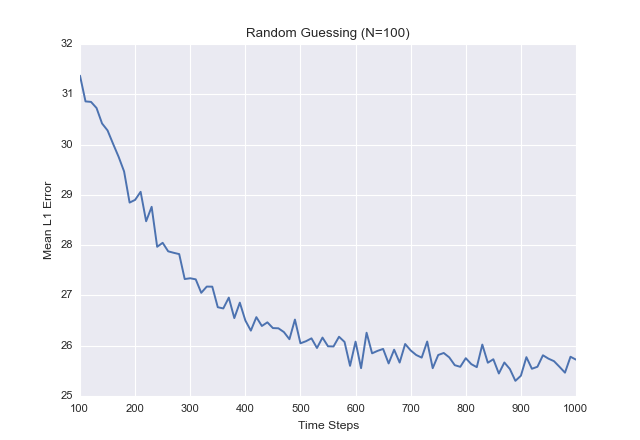
\includegraphics[width=0.5\textwidth]{figures/robustness/Random_Guessing21.png}%
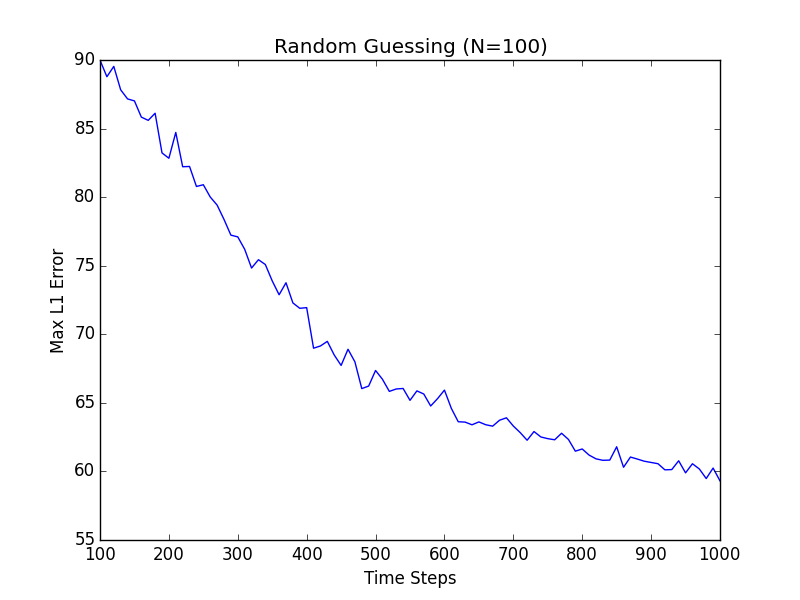
\includegraphics[width=0.5\textwidth] {figures/robustness/Random_Guessing22.png}%
}%
\caption{Mean and maximum $L_1$ error of Smarts Ratings when all $N$ players use a Random Guessing strategy. In Random Guessing, a player's Reported Guess is a random element from the domain of Smarts Ratings that is completely independent from the Actual Guess. These results establish baselines for subsequent simulations.}
\label{fig:RandomGuess}
\end{figure}

\subsubsection{Honest Play}

Honest players give Reported Guesses that are equivalent to their Actual Guesses. If all players are honest, Smarts Ratings quickly converge to Intelligences, as shown in Figure \ref{fig:HonestGuess}. Inducing honest play should be the foremost goal of LRS designers.

\begin{figure}[h]
\centerline{%
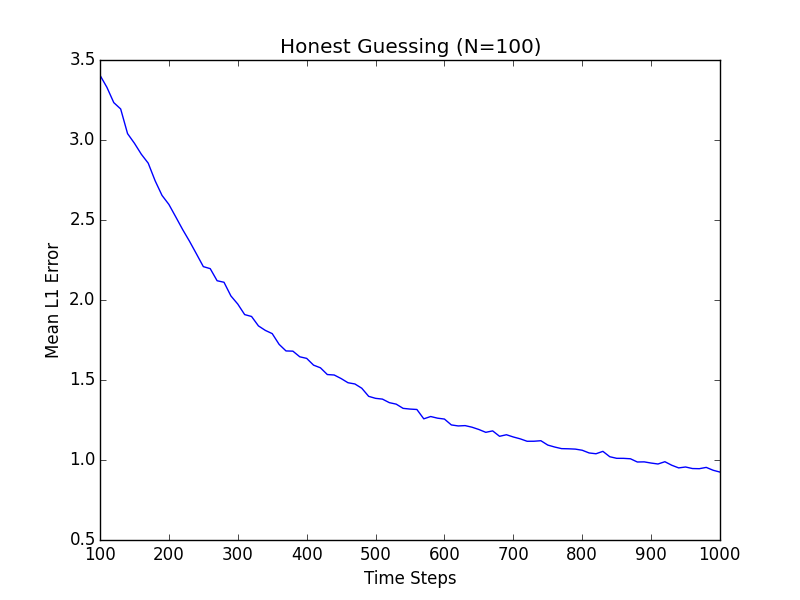
\includegraphics[width=0.5\textwidth]{figures/robustness/Honest_Guessing21.png}%
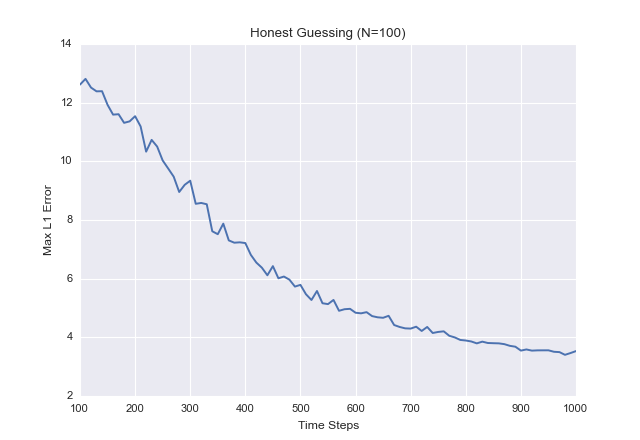
\includegraphics[width=0.5\textwidth] {figures/robustness/Honest_Guessing22.png}%
}%
\caption{Mean and maximum $L_1$ error of Smarts Ratings when all $N$ players Guess honestly. Honest play is defined by consistent equivalence between the player's Reported Guesses and Actual Guesses. Smarts Ratings quickly converge to intelligences if all players are honest.}
\label{fig:HonestGuess}
\end{figure}

\subsubsection{Single Priority Play}

If a player cares only about maximizing relative Smarts Ratings and neglects Luna Game outcomes, that player will likely give Reported Guesses of $0$ for all opponents. If all players use this Minimum Guessing strategy, Smarts Ratings will immediately collapse to $0$. More generally, the error introduced by Minimum Guessing depends linearly on the number of players using this strategy. Figure \ref{fig:MinimumGuess} confirms this result suggested by the theory. Mean $L_1$ error ranges from half the total range of Smarts Ratings to $0$.

\begin{figure}[h]
\centerline{%
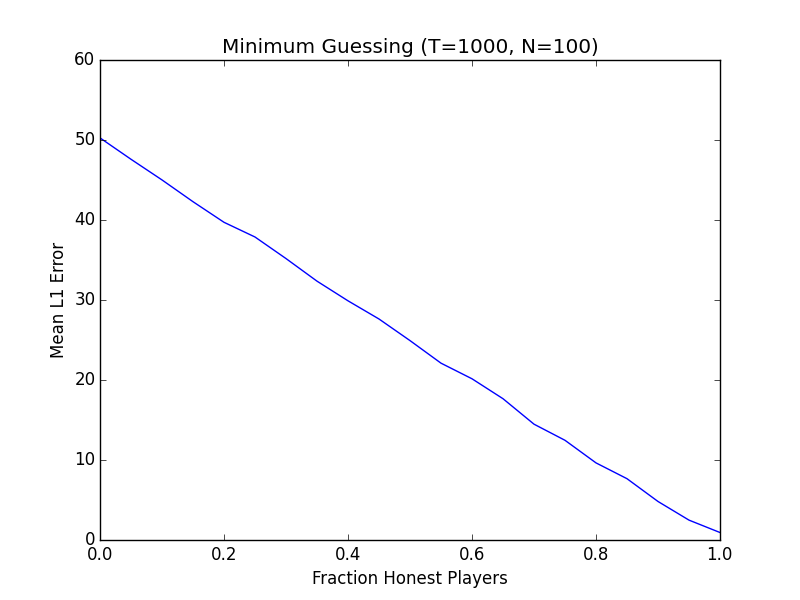
\includegraphics[width=0.5\textwidth]{figures/robustness/Minimum_Guessing31.png}%
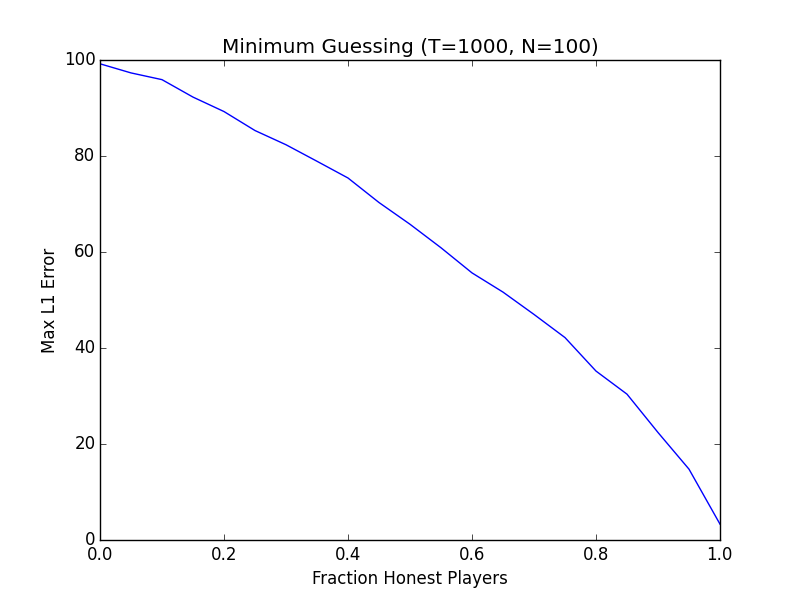
\includegraphics[width=0.5\textwidth] {figures/robustness/Minimum_Guessing32.png}%
}%
\caption{Mean and maximum $L_1$ error of Smarts Ratings when a fraction of the $N$ players use Minimum Guessing after $T$ time steps. In Minimum Guessing, a player always gives Reported Guesses of $0$. The error introduced by Minimum Guessing depends linearly on the number of players using the strategy.}
\label{fig:MinimumGuess}
\end{figure}

\subsubsection{Response Agnostic Play}

If the distribution of current Smarts Ratings is known at all times to all players, some players may try to take advantage of the distribution to formulate their guesses. A naive approach is to give Reported Guesses equal to the current mean Smarts Rating. With all players using this approach, the distribution collapses and error explodes. In general, Figure \ref{fig:MeanGuess} shows that the error introduced by Mean Guessing depends linearly on the number of players using the strategy.

\begin{figure}[h]
\centerline{%
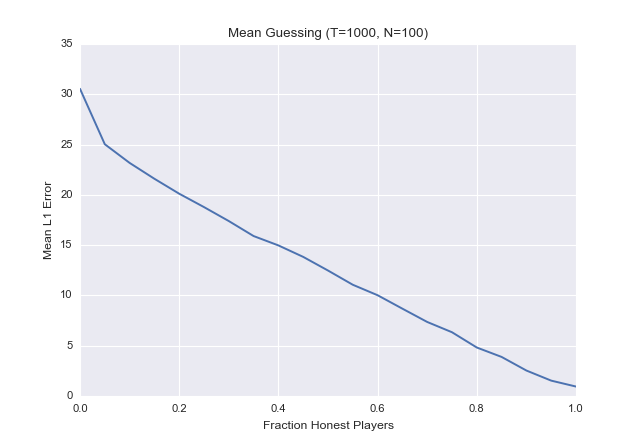
\includegraphics[width=0.5\textwidth]{figures/robustness/Mean_Guessing31.png}%
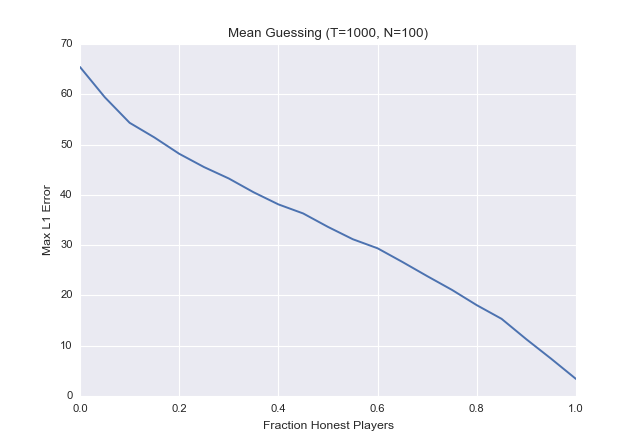
\includegraphics[width=0.5\textwidth] {figures/robustness/Mean_Guessing32.png}%
}%
\caption{Mean and maximum $L_1$ error of Smarts Ratings when a fraction of the $N$ players use Mean Guessing after $T$ time steps. In Mean Guessing, a player always gives Reported Guesses equal to the mean of all Smarts Ratings in the system. The error introduced by Mean Guessing depends linearly on the number of players using the strategy.}
\label{fig:MeanGuess}
\end{figure}

Another way that players may take advantage of a known distribution is via the Quantile Guessing strategy described above. The implementation of Quantile Guessing used for simulations uses the Empirical Cumulative Distribution Function with the sample composed of Actual Guesses of past opponents. A Reported Guess defaults to Actual Guesses if no Smarts Ratings have been determined, and for a player's first Luna Game. Ratings again collapse if all players use this strategy from the start, as shown in Figure \ref{fig:QuantileGuess}. 

\begin{figure}[h]
\centerline{%
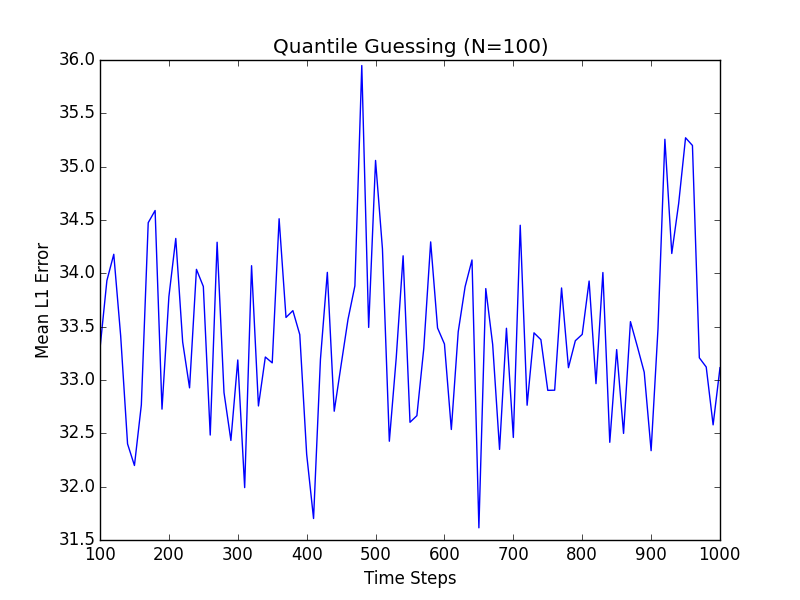
\includegraphics[width=0.5\textwidth]{figures/robustness/Quantile_Guessing21.png}%
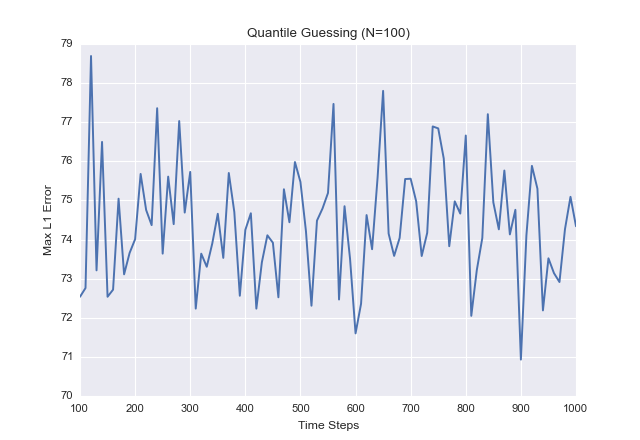
\includegraphics[width=0.5\textwidth] {figures/robustness/Quantile_Guessing22.png}%
}%
\caption{Mean and maximum $L_1$ error of Smarts Ratings when all $N$ players use Quantile Guessing. Quantile Guessing takes advantage of the distribution of all Smarts Ratings and a player's estimation of an opponent's rating percentile to formulate Reported Guesses. Due to the discrete nature of Smarts Ratings, Quantile Guessing causes Smarts Ratings to collapse to a constant, and the system cannot recover.}
\label{fig:QuantileGuess}
\end{figure}

If only a fraction of players use the strategy, the error depends linearly on the fraction, as was the case with Minimum and Mean Guessing. Figure \ref{fig:QuantileGuessFrac} confirms this result.

\begin{figure}[h]
\centerline{%
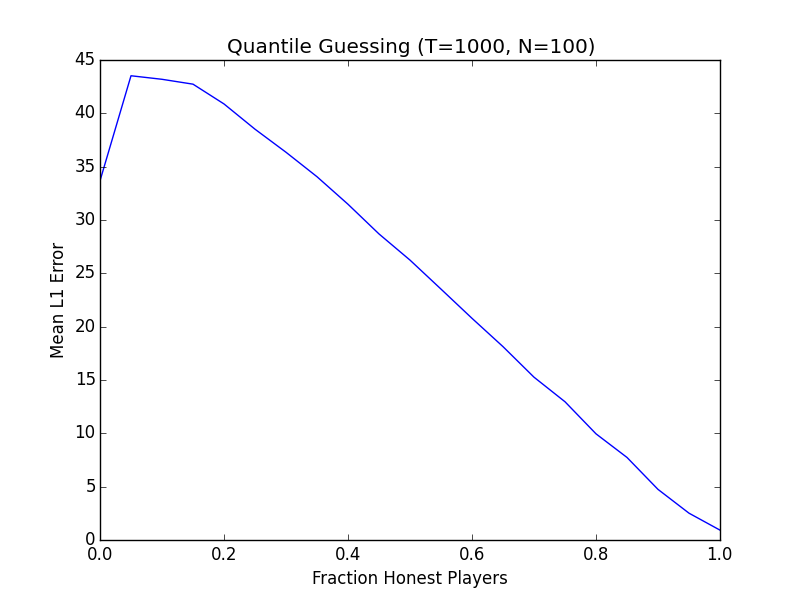
\includegraphics[width=0.5\textwidth]{figures/robustness/Quantile_Guessing31.png}%
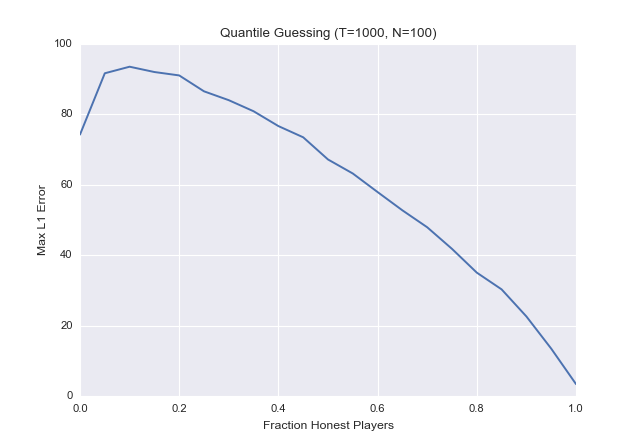
\includegraphics[width=0.5\textwidth] {figures/robustness/Quantile_Guessing32.png}%
}%
\caption{Mean and maximum $L_1$ error of Smarts Ratings when a fraction of $N$ players use Quantile Guessing after $T$ time steps. Quantile Guessing takes advantage of the distribution of all Smarts Ratings and a player's estimation of an opponent's rating percentile to formulate Reported Guesses. The error introduced by Quantile Guessing depends linearly on the number of players using the strategy.}
\label{fig:QuantileGuessFrac}
\end{figure}

What if the distribution is revealed once a certain number of games have been played? One might hope that the collapsing to a constant problem is avoided in this case. To test this hypothesis, the simulation in Figure \ref{fig:QuantileGuessDelay} introduces players that play with honest guessing for a variable number of time steps, and then play with Quantile Guessing for $500$ time steps. The delay in introducing Quantile Guessing does indeed improve the $L_1$ error within the time frame tested, though significant error remains after $500$ time steps for all tested delays. 

\begin{figure}[h]
\centerline{%
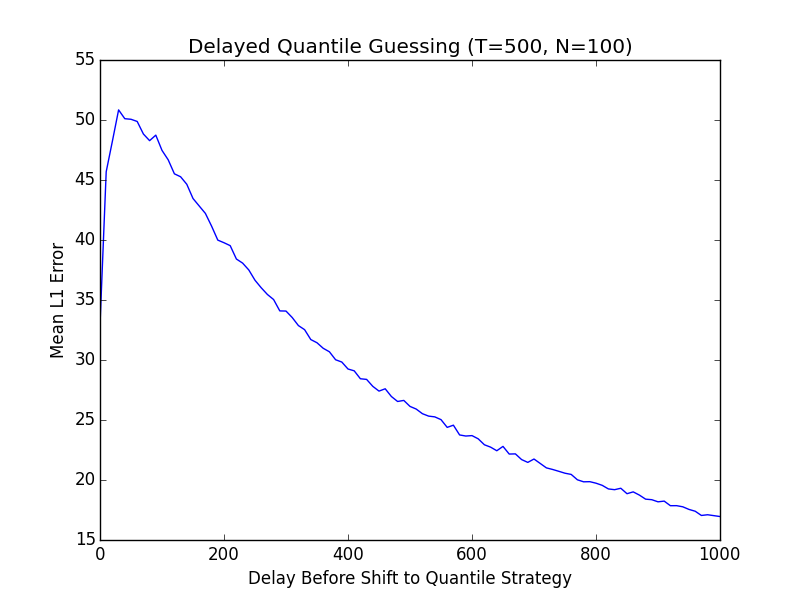
\includegraphics[width=0.5\textwidth]{figures/robustness/Delayed_Quantile_Guessing41.png}%
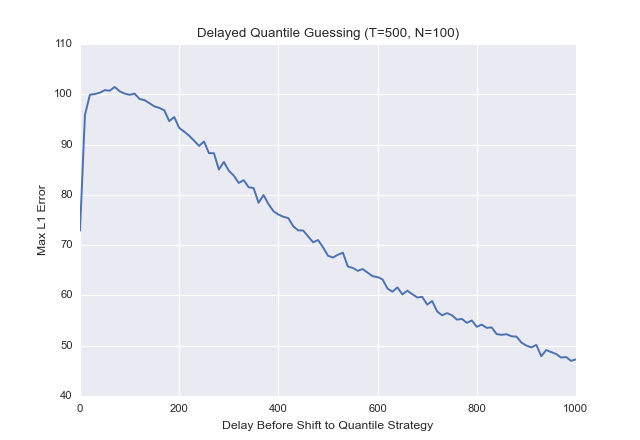
\includegraphics[width=0.5\textwidth] {figures/robustness/Delayed_Quantile_Guessing42.png}%
}%
\caption{Mean and maximum $L_1$ error of Smarts Ratings when $N$ players give honest guesses for some number of delay time steps, and then shift to the Quantile Guessing strategy for 500 additional time steps. The shift delay is negatively correlated with Quantile Guessing, suggesting that the negative impact of the strategy decreases if it is introduced after LRS has already stabilized.}
\label{fig:QuantileGuessDelay}
\end{figure}

\subsection{Combined Strategies}

In a real instantiation of LRS, it is unlikely that any single strategy will be adopted by all players. Thus the extreme results portrayed above are not of urgent concern. More likely is a situation where a small fraction of players adopt each of the strategies above. For the purpose of simulation, I assume that some fraction of players will play honestly, and the remaining players will be evenly divided among the strategies described above: Random Guessing, Minimum Guessing, Mean Guessing, and Quantile Guessing. Figure \ref{fig:Combined} shows that the relationship between error and honest player proportion is linear, as might be expected given the previous simulations. Roughly, for every additional $10$\% of players that forgo honest guessing in favor of one of the other strategies, the mean $L_1$ error increases by $3.5$.

\begin{figure}[h]
\centerline{%
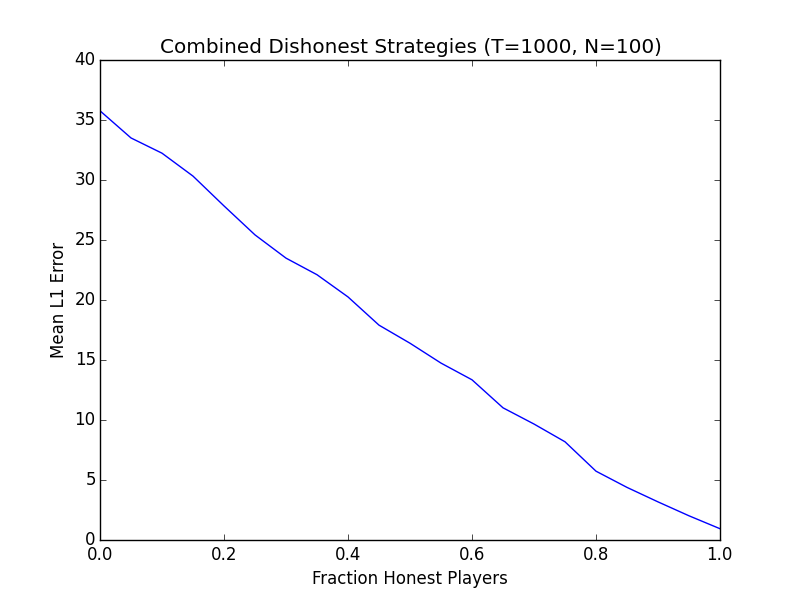
\includegraphics[width=0.5\textwidth]{figures/robustness/Combined_Dishonest_Strategies31.png}
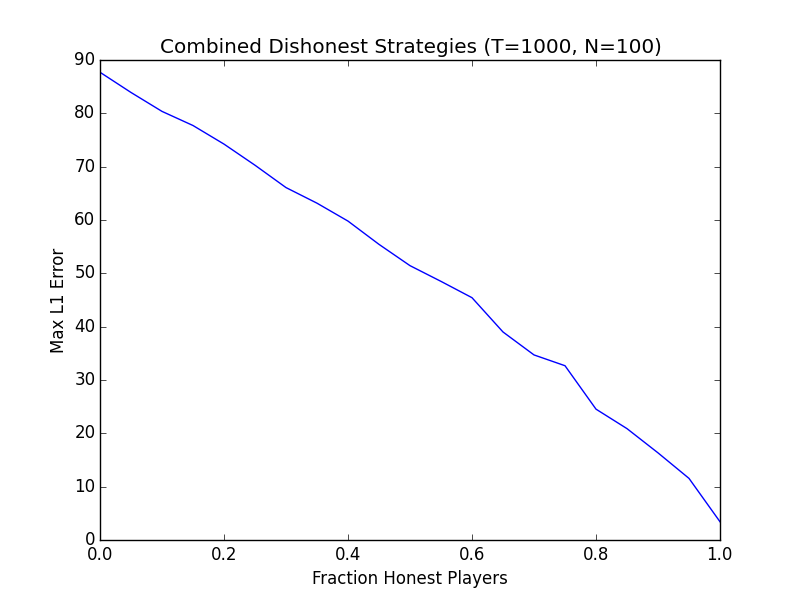
\includegraphics[width=0.5\textwidth] {figures/robustness/Combined_Dishonest_Strategies32.png}%
}%
\caption{Mean and maximum $L_1$ error of Smarts Ratings when some fraction of $N$ players give honest guesses, and the remaining players are split evenly among Random Guessing, Minimum Guessing, Mean Guessing, and Quantile Guessing strategies. The relationship between error and honest player proportion is linear.}
\label{fig:Combined}
\end{figure}
\section{Implications for LRS Design}

The theoretical and simulation results discussed in this chapter provide a cautionary tale for LRS designers. The system should be successful if all players practice honest play, but other strategies, such as Random Guessing, Minimum Guessing, Mean Guessing, and Quantile Guessing, threaten to undermine the validity of Smarts Ratings. Fortunately, these strategies can be grouped into two categories: strategies that are unlikely, and strategies that can be prevented. 

Random Guessing and Minimum Guessing belong in the unlikely strategy group. Random Guessing would be a bizarre long-term choice; the strategy gives a player no advantage in either Smarts Rating or Luna Game outcomes. Minimum Guessing is also unlikely for the player who realizes the personal benefit in terms of relative Smarts Ratings is very small. Minimum Guessing can also claim membership to the preventable strategy group; players practicing this strategy can be quickly identified by the system and banned for violating the spirit of play. Since they rely on the distribution of Smarts Ratings, Mean Guessing and Quantile Guessing are also easily avoidable; the distribution can simply be withheld from players. The distribution may also be withheld initially and introduced once the system has evolved and stabilized. This delay would improve Quantile Guessing for players, and these later players would introduce less error to Smarts Ratings by using the strategy.

If the Smarts Rating distribution is withheld from players, designers must choose another method for describing the ratings, or else the players will have no basis to form their first guesses. This chapter has discussed several avenues that should be avoided: fixed initializations of Smarts Ratings; a first-time ``quiz'' to initialize Smarts Ratings; or communicating only the average Smarts Rating. One option is to provide a vague disclaimer, such as ``Smarts Ratings are positive real numbers that typically range between $0$ and $100$.'' A more concrete alternative would be to ask players, ``On a scale from $0$ to $100$, how smart is your opponent?'' Of course, providing any numbers in the instructions encourages machine players to adopt Means Guessing or a similar naive strategy early on. Initializing these early Smarts Ratings is ultimately a chicken-or-egg problem that can only be resolved in practice by well-meaning human players.

The results in this chapter underscore the importance of good faith among players of the Luna Game. For researchers hoping to use LRS as a test of AI, the integrity of the system is essential if their own results are to be meaningful. Honest play is in the best interest of these players. Casual human players should also understand that dishonest strategies in mass can threaten both the validity and the distribution of Smarts Ratings, rendering LRS neither informative nor fun for players. The spirit of the Game should be made as clear to players as the limited attention span of Internet users permits. As with any test of human intelligence, LRS ultimately requires judges and subjects to play along.
